\section{Adam Wu}

\subsection{Github Setup and CI Checks}
I started working on setting up the Github and worked on building a CI checks, rulesets, and artifact for compiling our LaTeX file. This helps to ensure that the LaTeX file is always compiling during the development process. Furthermore, it prevents other members from pushing code that breaks the LaTeX file. 

\subsection{Design For Assembly}
On the design for assembly portion for submission 2, I worked on the CAD of the aesthetic prototype of the smart lock. I tried my best to make sure that the parts were designed in a way that they could be easily assembled and disassembled.

\begin{figure}[htbp]
    \centering
    \begin{subfigure}[b]{0.48\textwidth}
        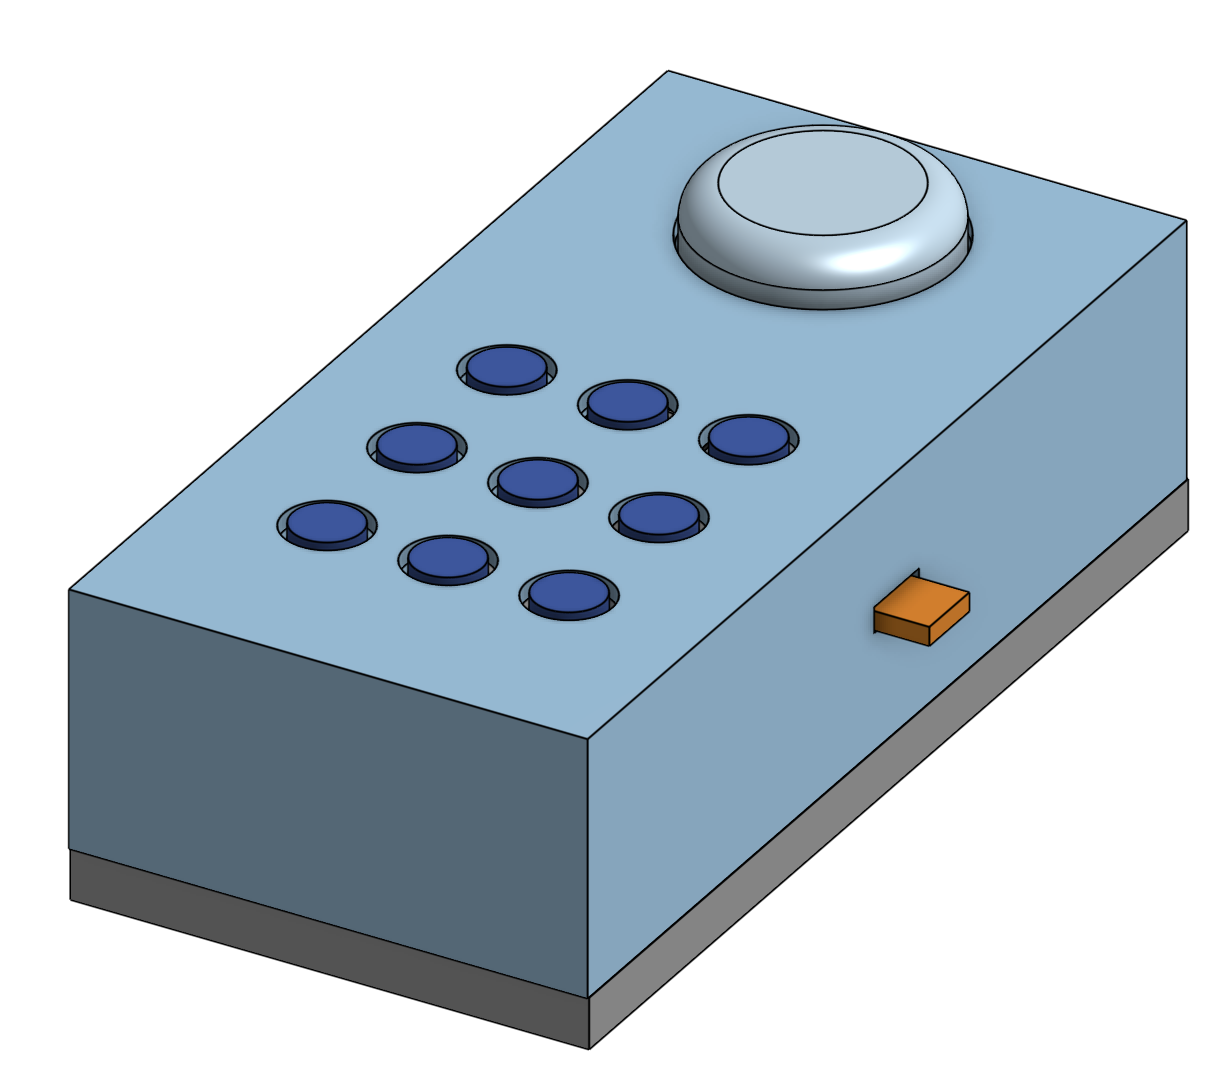
\includegraphics[width=\textwidth]{../submission3/img/isoView.png}
        \caption{Isometric View}
        \label{fig:isoView}
    \end{subfigure}
    \hfill
    \begin{subfigure}[b]{0.48\textwidth}
        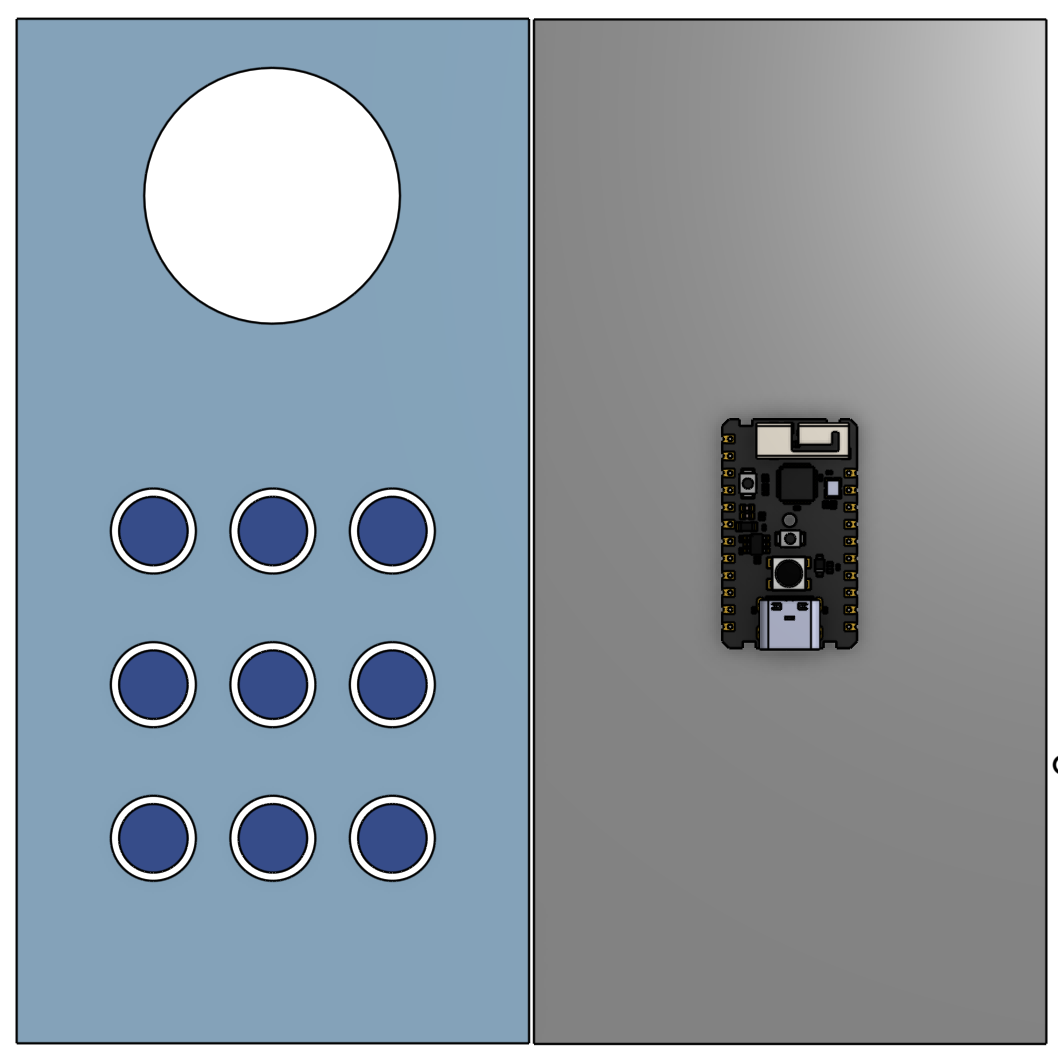
\includegraphics[width=\textwidth]{../submission3/img/topView.png}
        \caption{Top View}
        \label{fig:topView}
    \end{subfigure}
    \caption{First lock design}
\end{figure}

\subsection{Setting up ESP32-C3 toolchain (ESP-IDF)}
Since I am planning to work with the ESP32-C3, I started setting up the ESP-IDF toolchain on my local machine. I also started working on the initial setup of the ESP32-C3 to work with the "Hello World" example. Furthermore, I put in my researched information on the ESP-IDF documentation on where we can get started to connect to the WI-FI and to connect to Firebase.

\begin{enumerate}
    \item ESP-IDF have examples on basic wifi connection:
    \begin{itemize}
        \item in: \texttt{esp-idf/examples/wifi/getting\_started/station}
    \end{itemize}
    \item ESP-IDF also have examples on connecting to servers
    \begin{itemize}
        \item in: \texttt{esp-idf/examples/protocols}
    \end{itemize}
    \item We might also need to get another library for firebase connection
    \begin{itemize}
        \item link to firebaseClient: \url{https://github.com/mobizt/FirebaseClient}
        \item Another one: \url{https://github.com/dahmadjid/Firebase-idf}
    \end{itemize}
\end{enumerate}

\subsection{Gantt Chart}
For submission 2, I worked on the Gantt chart. I utilized a gantt chart template from a youtube video and modified it to fit our project. I also added the tasks that we need to complete for the next quarter.

\subsection{Test Plan}
I helped editing the test plans for ideas that was not put on the paper. I also helped with the formatting of the test plan.
